\documentclass[../main.tex]{subfiles}

\begin{document}

This chapter discusses the implementation details of the techniques used to crawl, extract and analyse the cookie banners in Greece as well as the UK. The implementation steps can be divided into 4 distinct steps which are summarised in the following list:

\begin{enumerate}
    \item \textbf{Identifying websites}: The methods and software developed to build a robust dataset of popular websites both in Greece and the UK and to deal with the issues faced from \say{local nuances};
    
    \item \textbf{Collecting the cookie banners}: The extension that was developed to allow OpenWPM to detect and collect cookie banners on the websites that it visits;
    
    \item \textbf{Normalising the data}: The methods and software used to identify the privacy options within the collected cookie banners and how they were classified based on the categories introduced in Table \ref{tab:privacy_options_categories};
    
    \item \textbf{Analysing data}: The techniques used to extract information from the collected data in order to answer the research questions set out by this project.
\end{enumerate}

\section{Identifying Websites}
The first step of the cookie banner collection process is to identify the most popular websites within Greece and the UK. However, while it might be trivial to single out websites that use each country’s TLD, identifying popular websites with different suffixes can be challenging. Furthermore, some websites explicitly refuse tracking or crawlers in their website and therefore, they have to be excluded from the dataset. Specifically, the first step can be subdivided into 3 sub-steps that are summarised in the following list:

\begin{enumerate}
    \item \textbf{Gathering the URLs}: The global, as well as local, ranking lists used and the software, developed to extract the links from those lists;
    
    \item \textbf{Compliance with robots.txt}: The novel method built and used by this project in order to comply with the Robots Exclusion Standard set by each website;
    
    \item \textbf{Compliance with Terms of Service}: The novel method developed by this project in order to make best efforts to comply with the terms and conditions of each website in the dataset.
\end{enumerate}

\subsection{Gathering links}
The primary focus of this project is to study cookie notices in Greek as well as UK websites. Therefore, it is essential to identify websites in both countries and ideally the most popular ones there in order to build a robust and diverse dataset.

For identifying the top websites in the target countries, this project utilised the Tranco list which was created by Le Pochat et al. Tranco, aggregates the top results from lists provided by Alexa (\url{https://alexa.com}), Cisco Umbrella (\url{https://umbrella.cisco.com/}), Majestic (\url{https://majestic.com/}), and Quantcast (\url{https://quantcast.com/}) and makes them available in a CSV format. In total, the Tranco list contains 1-million websites from across the world ordered by their rank.

\subsubsection{Filtering websites by their TLDs \& SLDs}
Both Greece and the UK have their own Top-Level Domain (TLD) which are .gr and .uk respectively. While Greece was also granted the \say{el} (or \say{.ελ} in Greek) TLD by IANA, after petitioning for years \cite{iana_el}, it has seen a low adoption by businesses and government agencies and therefore, it has not been taken into consideration in this project. Therefore, since each TLD is unique to a country, they can be used to find and retrieve websites from Tranco’s large dataset. 

Furthermore, Second-Level Domains (SLDs), such as .gov.uk, can also be used to enhance the filtering and also demonstrate the category that a website falls into. Thus, this project takes advantage of a wide range of Top and Second-Level Domains, in order to identify the websites in Greece as well as the UK. Table \ref{tab:impl_tlds}, summarises the TLDs and SLDs that are used to filter and retrieve websites from the Tranco list.

\begin{table}[ht]
\centering
\begin{tabular}{@{}lll@{}}
\toprule
\textbf{Greece} & \textbf{UK}     & \textbf{Description}                                     \\ \midrule
.gr             & .uk             & The Top-Level Domain for each country.                   \\
.com.gr         & .co.uk          & For private businesses and the commercial sector         \\
.gov.gr         & .gov.uk         & Used by local and federal government agencies            \\
.net.gr         & .net.uk         & Used by Internet Service Providers (ISPs)                \\
.org.gr         & .org.uk         & Primarily used by non-profit organisations               \\
sch.gr          & .sch.uk         & For educational authorities such as high schools         \\
                & .ac.uk          & Used by higher education institutes                      \\
                & .\{ltd/plc\}.uk & For Ltd or Plc companies                                 \\
                & .me.uk          & Personal names                                           \\
                & .nhs.uk         & Used by the NHS and its trusts                           \\
                & .police.uk      & For the UK police and its local forces                   \\ \bottomrule
\end{tabular}
\caption{The TLDs and SLDs for Greece \cite{gr_registar} and the UK \cite{nominet_additional_domains, nominet_rules} used to filter the Tranco list.}
\label{tab:impl_tlds}
\end{table}

\subsubsection{Dealing with local nuances}
However, it is not mandatory for businesses and other websites to use the conventional .gr or .uk suffix. Therefore, popular websites from each country that are using TLDs such as .com are missed when using the TLD as the only filter. 

For instance, Aegean Airlines (\url{https://en.aegeanair.com/}) is the largest Greek airline, providing domestic, as well as international flights, to and from a large number of airports across the world. Although it is a Greek business, since they are operating globally they are using the popular .com suffix to provide a more familiar domain name to international customers and therefore, attract more business. Thus, although Aegean is in the Tranco list, due to the fact that they use a .com domain will be missed if a simple TLD/SLD clarification is used.

For tackling the local nuances discussed above, additional lists have been used to aid the original Tranco list. These lists rank the most popular websites within a certain country without taking into consideration their TLD. More specifically, these lists are:

\begin{itemize}
    \item \textbf{TopGR} (\url{https://topgr.gr}): Provides a list of the most visited Greek websites, based on their Alexa rankings;

    \item \textbf{Kadaza} (\url{https://kadaza.co.uk}): Provides the 24 most popular websites in the UK in a wide range of categories such as news, shopping and travel. The list is manually curated by the Kadaza team by \say{monitoring the latest website traffic data and local website trends};

    \item \textbf{Finder.com} (\url{https://finder.com}): Compares online online retailers and services for a number of different categories such as beauty, fitness, energy providers, mortgages etc. Finder.com manually curates its lists and updates them daily in order to ensure best quality. Because of the rise of online shopping due to the Coronavirus pandemic \cite{skeldon_2020, columbus_2020}, ensuring that all major retailers are included in this study is essential. Therefore, Finder provided a reliable source for finding UK online retailers. 
\end{itemize}

While the above lists have not been used as the primary source for building the dataset, they provide a good solution on the issue of local nuances and they also provide a more diverse set of websites that may have never been studied before.

\subsubsection{Building the dataset}
In order to build the dataset, a Python3 script was developed that applied the TLD/SLD filter on the Tranco list and also parsed the additional lists. The script takes 3 steps to build the dataset, which is summarised in the following list:

\begin{enumerate}
    \item \textbf{Build the TLD set}: The script parses the Tranco list and builds a set that contains all the websites with the specific suffix (e.g: .gr);

    \item \textbf{Build the local set}: The script parses the additional lists (e.g. TopGR) and builds a set containing the websites from there;

    \item \textbf{Merge the two sets}: The script merges the two sets. The final set contains the original set (e.g all the .gr domains) and the items of the second set that also exist in the Tranco list. 
\end{enumerate}

% The above can be expressed more formally in set theory notation. Assume that A is the set containing all the URLs in the Tranco list, B is a strict subset of A that contains the .gr domains and C is set containing all the TopGR URLs. Thus, we have that the script returns all the URLs where:

% \[ B \cup (A \cap C) \]

Finally, the remaining websites are stored in an SQLite database in order to be easily accessible for further analysis. SQLite was chosen for the purposes of this project since it provides a fast and reliable SQL database implementation. However, the most important feature of SQLite is that it is self-contained and therefore, the database file can be easily shared and accessed, without the need for an SQL server. The source code for the above script can be found in Appendix \ref{app:code_design_websites_lists}.

\subsection{Compliance with the Robots Exclusion Standard}
The Robots Exclusion Standard, or simply known as robots.txt, can be used by websites to specify which parts of the website should not be processed by web crawlers and robots \cite{koster_1994}. Robots are used by search engines for categorisation purposes but can also be used by competitors to retrieve information about the website. Therefore, website administrators can choose to exclude certain directories from crawlers as shown in Figure \ref{fig:design_example_robots}. 

\begin{figure}[ht]
    \centering
    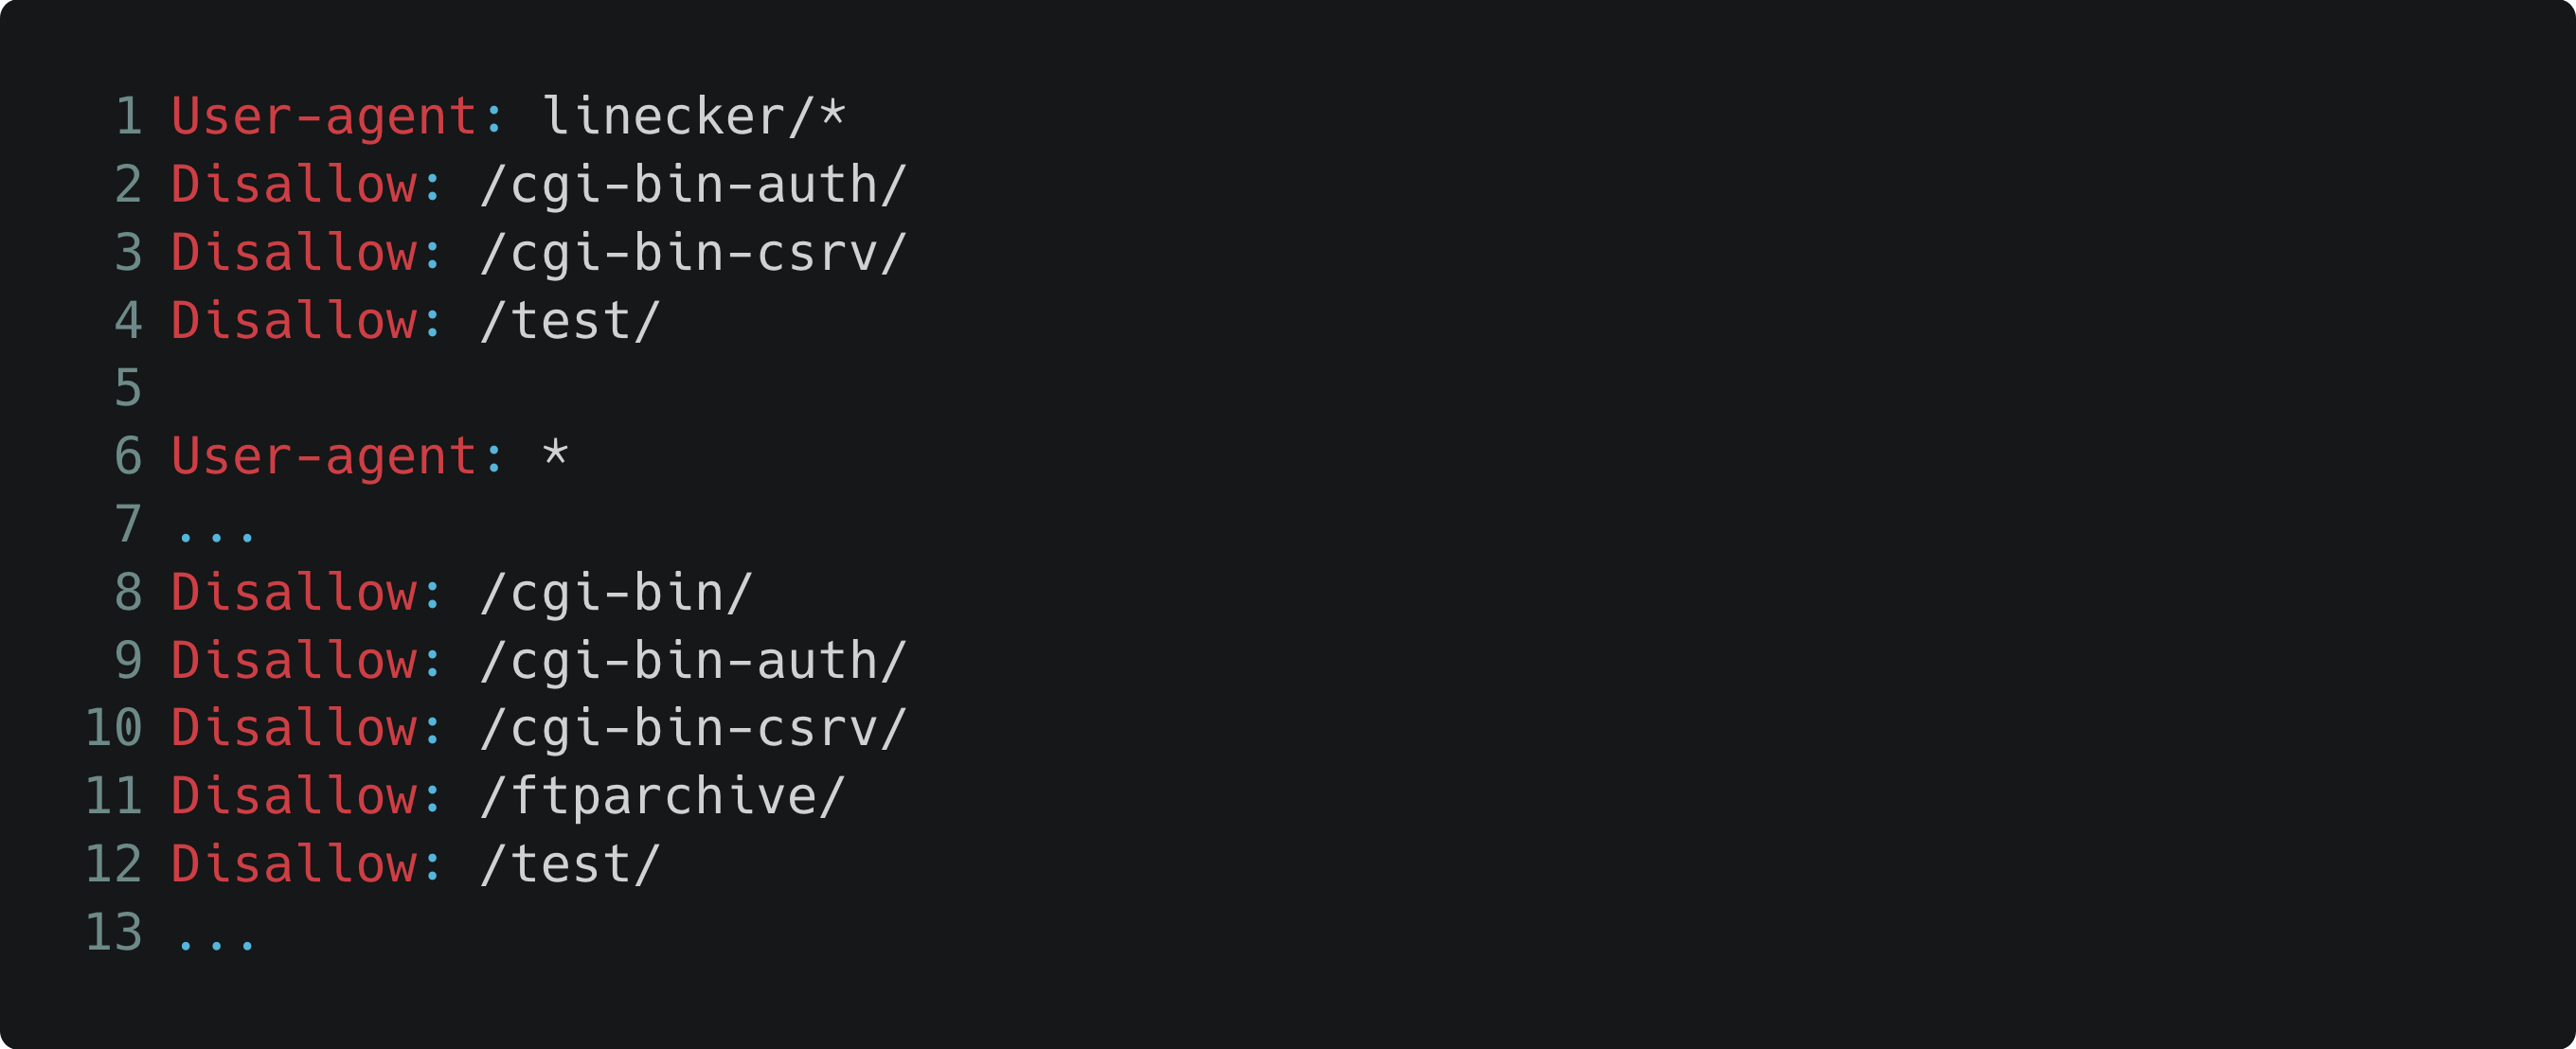
\includegraphics[width=\textwidth]{images/implementation/example_robots.png}
    \caption{Parts from the York University robots.txt file (\url{https://york.ac.uk/robots.txt}) that uses the Disallow keyword to stop crawlers from processing that part of the website.}
    \label{fig:design_example_robots}
\end{figure}

Since the software built and used for detecting cookie banners resembles a crawler, this project aimed to respect the exclusion standard set out by the websites. To do so, a Python3 script was built that parses robots.txt files and verifies whether they allow crawling. That script was applied to the dataset that was built on the first step.

More specifically, the script verifies that a robots.txt exists and it allows crawlers to parse the root directory of the website, otherwise the website is marked as \say{not-crawlable} as it can be seen in Listing \ref{lst:design_robots}.

\begin{lstlisting}[language=Python, caption=Pseudocode of the algorithm followed by the robots.txt parser script., label=lst:design_robots,captionpos=b, style=lst_style]
For every $website in the dataset:
    Find the robots.txt file of $website
    If robots.txt does not exist:
        Mark $website "uncrawlable"
    
    If robots.txt allows crawling:
        Mark $website "crawlable"
    Else:
        Mark $website "uncrawlable"
\end{lstlisting}

The script utilises the reppy Python library \cite{reppy} that aids with parsing and analysing the robots.txt of a website. Furthermore, it has been parallelised using Python’s multiprocessing library in order to take advantage of every available CPU core in the system and reduce runtimes. Finally, the SQLite database containing the dataset is updated to reflect the crawl status of each website. The source code for the robots.txt compliance script can be found in Appendix \ref{app:code_design_robots}.

\subsection{Compliance with the Terms of Service}
In addition to the Robots Exclusion Standard, this project makes best efforts to comply with the Terms of Service (TOS) of the websites within the dataset. This was done for two reasons:

\begin{enumerate}
    \item Some websites use default or auto-generated robots.txt file that allows crawlers to visit their website. However, on their TOS they specifically state that they do not want robots scraping their content;
    
    \item The cookie banner detector software developed for this project collects the HTML of the cookie notices found in websites, which can be considered content. Some websites explicitly state that their content is aimed for personal use only. 
\end{enumerate}

The exclusionary terms were selected after manually reading over 50 TOSs, from websites in both countries, and finding the most common wording that websites use for prohibiting visitors from using the website, as well as its content, in a not-acceptable manner. A number of different terms and phrases both in English as well as Greek were identified, such as \say{for personal use only} which are summarised in Table \ref{tab:design_tos_terms}.

\begin{table}[ht]
    \centering
    \begin{tabular}{@{}ll@{}}
        \toprule
        \textbf{Greek Phrases}    & \textbf{English Phrases} \\ \midrule
        Strictly for personal use & Personal use only        \\
        Only for personal use     & Only for personal use    \\ \bottomrule
    \end{tabular}
    \caption{The English as well as Greek phrases (translated) that the Terms of Service parser use. The original Greek terms can be found in \ref{tab:impl_greek_exclusion_terms}.}
    \label{tab:design_tos_terms}
\end{table}

A Python3 script was developed that makes best efforts to ensure TOS compliance. More specifically, the script visits a website and looks for a TOS link. If a link is found, it visits the Terms of Service page and examines its text for terms or phrases that may indicate that the website refuses to be tracked. The algorithm used by the script is shown in Listing \ref{lst:design_tos}.

\begin{lstlisting}[language=Python, caption=Pseudocode of the algorithm that the Terms of Service parser uses., label=lst:design_tos,captionpos=b, style=lst_style]
For every $website in dataset And robots.txt allows crawling:
    If $website has TOS link:
        Go to the TOS page
        If TOS page has exclusionary terms:
            Mark website "uncrawlable"
        Else:
            Mark website "crawlable"
    Else:
        Mark website "crawlable"
\end{lstlisting}

The Terms of Service parser uses Python’s \say{request} library to navigate to websites and BeautifulSoup4 \cite{richardson2007beautiful}, a library that provides easy and efficient programmatic access to HTML elements. More specifically, the steps are taken by the TOS parser are summarised in the following list:

\begin{enumerate}
    \item \textbf{Visit the website}: Using Python’s request library, the script makes a simple GET request to the URL and it pulls its HTML code for analysis;
    
    \item \textbf{Look for a TOS link}: The HTML code is then parsed by BeautifulSoup. The script looks for anchor elements (<a>) that might link to a Terms of Service page by searching for specific terms which are listed in Table \ref{tab:tos_phrases};

    \item \textbf{Go to TOS page}: If such a link is found, then the script pulls the HTML code from the TOS page and it feeds it to the HTML parser as before;

    \item \textbf{Look for exclusionary terms}: The script searches the Privacy Policy text for specific exclusionary terms from Table \ref{tab:design_tos_terms}.
\end{enumerate}

Finally, the script updates the crawl status of each website in the dataset. The full source code of the Terms of Service parser can be found in Appendix \ref{app:code_design_tos}.

\section{Detecting Cookie Banners}
After the dataset has been built, the next step is to visit the candidate websites that allow crawling. In order to do so, this project uses OpenWPM and extends it by giving it cookie banner detection capabilities. More specifically, detecting cookie banners can be split into two sub-steps which can be summarised as follows:

\begin{enumerate}
    \item \textbf{CSS Selectors}: Build a list of common CSS selectors that are used by cookie banners across Greece and the UK;

    \item \textbf{Extend OpenWPM}: Give open OpenWPM cookie banner detection capabilities and scrape the dataset with the aid of the CSS Selectors list that was built before; 

    \item \textbf{Data collection}: Collect the cookie banners and their attributes for later analysis.
\end{enumerate}

\subsection{I don't care about cookies}

The GDPR requires websites to seek the users’ permission before installing tracking cookies on their web browser. However, if users surf the web anonymously then the same websites will ask for the user’s permission again. \say{I don’t care about cookies} (IDCAC) is a popular web browser extension that removes the cookie notices and saves the user \say{thousands of unnecessary clicks}. 

In order to remove those notices, IDCAC has built a list of CSS selectors that websites use for their cookie notices. For example, Figure \ref{fig:design_skyexpress} depicts the HTML of a cookie banner found in SkyExpress, a popular Greek airline (\url{http://skyexpress.gr}). Notice that it has an \say{id} attribute which is set to \say{cookie-notice}. Thus, if the IDCAC list contains the CSS selector {\fontfamily{pcr}\selectfont \#cookie-notice}, the extension can effectively hide the cookie banner.

\begin{figure}[ht]
    \centering
    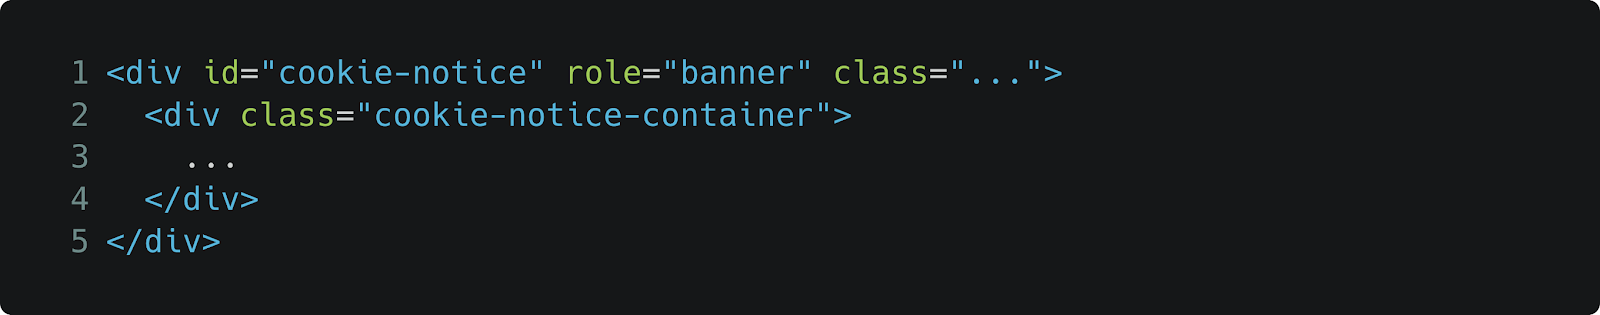
\includegraphics[width=\textwidth]{images/implementation/skyexpress.png}
    \caption{The HTML of the cookie banner found in SkyExpress.}
    \label{fig:design_skyexpress}
\end{figure}

A similar technique was used by Eijk et al. when studying the cookie banners on their dataset. However, the implementation of the IDCAC parser developed for this project differs significantly. The following list summarises the steps that are taken to parse the IDCAC as well as their differences between this project and Eijk et al. approach:

\begin{enumerate}
    \item \textbf{Download}: Retrieve a fresh copy of the \say{I don’t care about cookies} list from their website (\url{https://www.i-dont-care-about-cookies.eu/abp/}), to ensure that no new CSS selectors are missed. While Eijk et al. download and parse the IDCAC list every time their code is executed, this project processes the IDCAC list in a separate script (or a different sub-step) and adds the CSS selectors in a database. This was done for 2 reasons. Firstly, the IDCAC list is not updated regularly and therefore, there is no point in downloading it and parsing it every time the code is executed. Secondly, the set of websites parsed by OpenWPM are almost always the same and therefore, it is unlikely that OpenWPM will have to deal with different CSS selectors and cookie notices at every run;
    
    \item \textbf{Parse}: Remove any unnecessary lines, comments or syntax around the CSS selectors and keep only the required content from the list. The IDCAC cookie parser implemented for this project is significantly optimised for better performance compared to the one introduced by Eijk et al. For instance, they use Python’s split method \cite{python_str_doc} to process different parts of the IDCAC list which can have a worst-case performance of $O(n)$. On the other hand, this project’s parser takes advantage of Python’s string cutting and slicing, which has a performance of $O(1)$. This can have a significant impact when processing over $16,000$ CSS elements;
    
    \item \textbf{Save}: Store the CSS selectors in a database for caching purposes, as well as easy access, by other applications such as OpenWPM, as discussed above.
\end{enumerate}

The IDCAC about cookies list has been enriched with an additional 64 CSS cookie banner selectors that were identified while testing the code of this project. While these 64 CSS selectors only account for 0.4\% of the IDCAC list, without them at least 400 Greek websites would have been missed, including online retailers and government agencies. These additional CSS selectors have been submitted to the IDCAC project in order to be added to the final list and improve IDCA's reach in Greece. The full source code of the IDCAC parser and the additional CSS selectors can be found in Appendix \ref{app:code_idcac_parser}. 

\subsection{Making OpenWPM care about cookies}
OpenWPM is an open-source tool, developed by Englehardt and Narayanan. It allows researchers to automatically measure Third-Party Cookies, trackers, cookie synchronisation as well as fingerprinting techniques, in websites.

Unfortunately, OpenWPM has no way of detecting the existence of cookie notices on the websites that it visited. Therefore, this project has developed a novel way of extending the functionality of OpenWPM in order to effectively detect cookie banners and store relevant information about them. 

More specifically, for each website OpenWPM checks whether it contains a CSS selector from the cached IDCAC list, using Selenium \cite{selenium}, which allows for searching the HTML code of the website. Once a selector has been identified, additional checks are made to ensure that this is not a false-positive. These additional checks are summarised in the following list: 

\begin{enumerate}
    \item \textbf{Selenium check}: Ensure that Selenium returned valid HTML e.g. the length of the HTML;
    \item \textbf{Cookie check}: Verify that the HTML returned by Selenium contains the terms \say{cookie} or \say{cookies}.
\end{enumerate}

If the cookie banner has been successfully identified, then it is stored in a database for further analysis. The combination of the cached cookie selectors and Selenium’s efficient DOM \cite{wood1998document} search enables the cookie banner extension to be fast, efficient and fault-tolerant. 

Listing \ref{lst:design_openwpm_steps}, summarises the novel steps added to OpenWPM in order to detect the cookie banners.

\begin{lstlisting}[language=Python, caption=Pseudocode of the steps that the OpenWPM extension uses., label=lst:design_openwpm_steps,captionpos=b, style=lst_style]
For every $website in dataset:
    Visit $Website
    If $website has CSS selector:
        Get cookie banner HTML
        Ensure not false-positive
        Save cookie banner
        Move to the next website
\end{lstlisting}

Furthermore, the cookie banner extension developed for this project is vastly different from the one developed by Eijk et al. for the purposes of their study. Specifically, the differences between the two extensions are summarised in the following list:

\begin{enumerate}
    \item \textbf{Searching for a cookie banner}: Eijk et al. search each website for every CSS selector on their list. Thus, if they have n CSS selectors, they perform n iterations and DOM searches (which can also be expensive) on each website, even if the correct CSS selector has already been found. This was probably done to eliminate false-positives (e.g. a selector matched an element that is not a cookie banner). On the contrary, the cookie banner detection implementation for this project stops when the first CSS selector matches an element, potentially saving thousands of unnecessary loops per website. During testing, and also when running the experiment on the full set of websites, the number of false-positives was not significant enough to justify the performance hit of an exhaustive search and those \say{edge} cases were fixed manually;
    
    \item \textbf{Data output}: This project outputs significantly more information and data for later analysis compared to Eijk et al. In addition to the cookie banners’ source code, the full website source code, as well as screenshots, are saved which can help when analysing the cookie banners.
\end{enumerate}

In total, the cookie banner extension consists of 7 files across the existing OpenWPM project. Table \ref{tab:impl_openwpm_files}, summarises these files, their purpose and source code.

\begin{table}[ht]
\centering
\begin{tabular}{@{}lll@{}}
\toprule
\textbf{File}              & \textbf{Description}                                        & \textbf{Code}       \\ \midrule
CookieBanner.py            & Cookie banner representation           & \ref{app:code_openwpm_cookie_banner}     \\
CommandSequence.py         & OpenWPM API to allow users to          & \ref{app:code_openwpm_command_sequence}  \\
                           & call cookie banner extensions          &                                          \\
Types.py                   & The types of commands                  & \ref{app:code_openwpm_types}         \\
browser\_commands.py       & The cookie banner detection            &                                          \\
                           & implementation                         & \ref{app:code_openwpm_browser_commands}  \\
command\_executor.py       & Works with CommandSequence             & \ref{app:code_openwpm_command_executor}  \\
                           & to call the right methods              &                                          \\
cookie\_utils.py           & Helper methods to aid cookie           & \ref{app:code_openwpm_cookie_utils}      \\
                           & banner detection                       &                                          \\
openwpm\_cookie\_parser.py & A script that prepares and starts      & \ref{app:code_openwpm_starter}           \\
                           & OpenWPM                                &                                          \\ \bottomrule
\end{tabular}
\caption{The files extended to allow OpenWPM to detect cookie banners.}
\label{tab:impl_openwpm_files}
\end{table}

\subsection{Data Gathering}
In addition to the cookie banner detection capabilities, the data gathering capabilities of OpenWPM were also enhanced as part of this project. More specifically, after a cookie banner is detected, a number of its attributes, as well as its source code, are stored in a database for further analysis. The information gathered per cookie banners include:

\begin{itemize}
    \item A boolean value that indicates whether a cookie banner was found for a given website;
    \item The size and position of the cookie banner;
    \item The HTML source code of the cookie banner;
    \item The CSS selector that was used to identify the notice, 
\end{itemize}

Figure \ref{fig:impl_openwpm_sample_data}, shows sample data collected by two websites using the cookie banner extension. Moreover, a screenshot, as well as the entire HTML code, is saved for every website. This is done in order to manually inspect errors or false-positives that may occur during the runtime of OpenWPM.

\begin{figure}[ht]
    \centering
    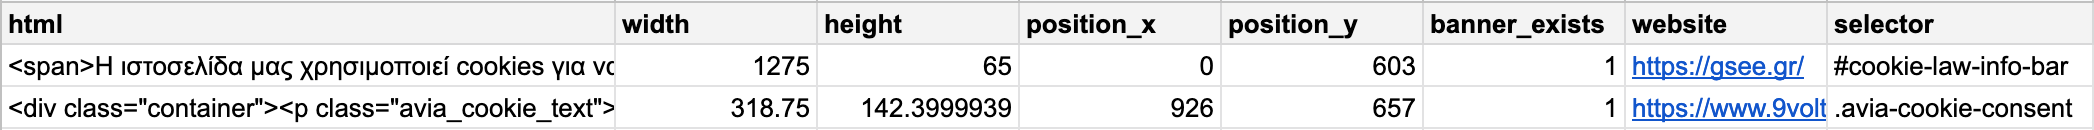
\includegraphics[width=\textwidth]{images/implementation/open_wpm_out.png}
    \caption{Sample data gathered after OpenWPM has finished running.}
    \label{fig:impl_openwpm_sample_data}
\end{figure}

\section{Sanitising \& Normalising the Data}
Throughout its execution, the OpenWPM cookie banner detector stores a plethora of data. However, given the amount of data and their particular structure, it can be challenging to efficiently query and analyse them. To tackle those issues, the following steps have been taken in order to make the data easier and more efficient to search: 

\begin{enumerate}
    \item \textbf{Identify actions}: Determine the \say{call to action} words used in the options offered by the cookie banners. For instance, distinguish the affirmative options such as \say{Accept} or \say{Ok} from the negative options such as \say{Decline} or \say{No}.
    
    \item \textbf{Structure data}: Having identified the options provided by the cookie banners, the collected data from the previous step can be converted from an arbitrary HTML format to a structured table-like format which allows for easier querying. 
\end{enumerate}

\subsection{Identifying Actions}
The first step of normalising the data is to determine the options that cookie banners provide and their different variations. The cookie banner options categories are the affirmative, non-affirmative, informative and managerial as they were introduced in Table \ref{tab:privacy_options_categories}.

In order to categorise the privacy options from the collected data, a Python3 script was developed. More specifically, the script looked at the HTML of each individual cookie banner, stripped it from all the unnecessary HTML tags and kept only the {\fontfamily{pcr}\selectfont <a>} and {\fontfamily{pcr}\selectfont <button>} tags. This was done because the overwhelming majority of privacy options (almost 100\% in the dataset) are programmed using those tags for 2 reasons. Firstly, they are easily identifiable by the users and know that they can interact with them. Secondly, it is easy for developers to detect when users have clicked such an element and run additional code. As a final step, the text within those tags, which is also known as \say{call to action}, was stored in a simple SQL table.

After the above script finished running, the SQL table and its entries were manually inspected and classified into the 4 cookie banner option categories. While this project aims to automate the entire process of detecting and classifying cookie banners, manual inspection of the privacy options and their call to actions can be beneficial and in some cases unavoidable.

Similarly to when identifying popular websites for a country, call to action phrases can hide local nuances. For instance, the majority of cookie banners collected from Greece had the noun \say{αποδοχή} (I accept) as their affirmative call to action. However, a large number of them used the verb \say{δέχομαι} which also means \say{I accept} as an affirmative call to action. 

It is clear that two different words can have the exact same meaning and therefore, a generic program or someone without an understanding of the language and its nuances can easily fail to classify the privacy options properly. Thus, manual intervention and classification, instead of an automated program, was decided for this step in order to avoid missing valuable information from an already rich dataset. 

\subsection{Structuring the Data}
After all the phrases and call to actions have been properly categorised, the arbitrary data collected by OpenWPM can be converted into an easy to search data structure. More specifically, the goal of this step is to take the HTML code collected from the cookie banners of each website and turn it into a SQL-like table that allows for efficient queries, without losing the core information included in the cookie banners. Converting the inconsistent structure of HTML into a structured format can yield the following benefits when analysing the data:

\begin{enumerate}
    \item \textbf{Accessibility}: Knowledge of HTML is not required when querying the data and therefore, the data can be imported in more popular applications such as Microsoft Excel;
    
    \item \textbf{Efficiency}: Faster interpretation and understanding of the data as they are displayed in a tabular format with consistent fields instead of arbitrary HTML code;
    
    \item \textbf{Searchability}: Efficient queries using tools such as SQL or Excel’s queries, instead of having to programmatically parse HTML code, which can be extremely inefficient and inconsistent.
\end{enumerate}

In order to convert the data to the table-like structure discussed above, a Python3 script was developed and its source can be found in Appendix \ref{app:code_options_parser}. More specifically, the script uses BeautifulSoup’s API to extract every privacy option from the cookie banner and then categorised them accordingly. Once a category has been identified the call to action is stored in the database and the cookie banner is marked to indicate that it contains that category. For instance, if a cookie banner has a button with a call to action \say{Accept}, then its database entry shows that it has an affirmative option. The algorithm described here is shown in Listing \ref{lst:impl_options_parser}.

\begin{lstlisting}[language=Python, caption=Pseudocode of the algorithm followed by the Cookie Banner Options parser., label=lst:impl_options_parser,captionpos=b, style=lst_style]
For every $cookie_banner in the database:
    For every $privacy_option in $cookie_banner:
        If $privacy_option is affirmative:
            Set $cookie_banner has affirmative option
            Save call to action
        If privacy_option is non-affirmative:
            Set $cookie_banner has non-affirmative option
            Save call to action
        ... (Same for informative and managerial categories)
\end{lstlisting}

Finally, the script also saves the privacy text that is displayed on the cookie banner, using a similar technique as above. More specifically, using BeautifulSoup it strips the cookie banner from all the unnecessary HTML tags (e.g. {\fontfamily{pcr}\selectfont <a>}, {\fontfamily{pcr}\selectfont <button>}, {\fontfamily{pcr}\selectfont <img>} etc.) keeping only the ones that are used for text such as {\fontfamily{pcr}\selectfont <p>}, {\fontfamily{pcr}\selectfont <span>} etc. Figure \ref{fig:impl_privacy_options_normalised}, depicts the table-like format that is produced after the script has finished executing. 

\begin{figure}[ht]
    \centering
    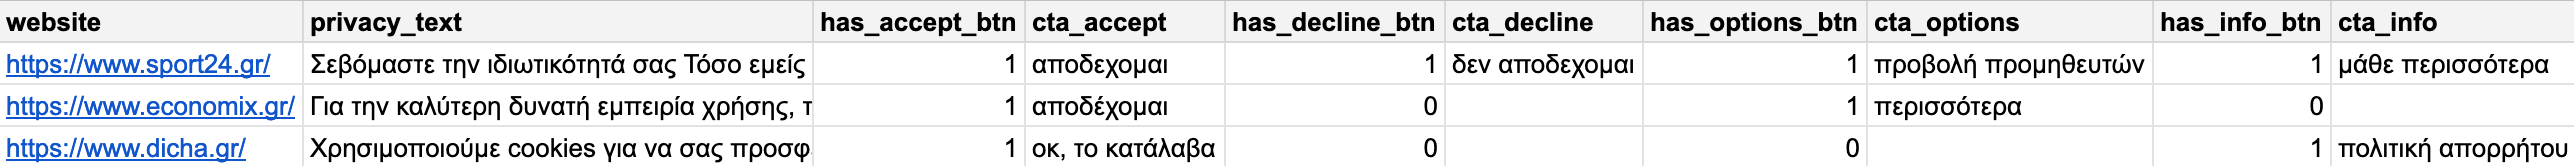
\includegraphics[width=\textwidth]{images/implementation/normalised_data.png}
    \caption{Normalised data after the Privacy Options parser has finished running.}
    \label{fig:impl_privacy_options_normalised}
\end{figure}

\section{Querying the Data}
After the data has been normalised, it can then be searched in order to answer the research questions. While the normalised data can be extracted to a spreadsheet and open by an application such as Microsoft Excel, this project retained the data in the original database in order to take advantage of SQL’s advanced search capabilities. The following list summarises the types of queries that have been developed to retrieve the required data: 

\begin{enumerate}
    \item \textbf{SQL queries}: Standard SQL queries, such as SELECT, that allow easy and efficient querying of the data in the database;
    
    \item \textbf{Python queries}: Where SQL fails to provide adequate representation of the data, Python has been used to compensate for those queries.
\end{enumerate}

\subsection{Querying with SQL \& Python}
The primary goal of Step 3 was to structure the collected data into an easy-to-query data structure. This can be achieved by using standard SQL syntax \cite{bowman1996practical} and most research questions have been answered using that. 

However, there are instances where SQL cannot handle the types of calculations required to answer some of the research questions. Those instances have been handled by implementing the queries using Python. For example, Questions 2 and 3 required a more advanced representation of the data and it would have been challenging to achieve those results using SQL and therefore, Python was used instead. Table \ref{tab:impl_rqs_sc}, summarises the scripts that were developed to answer the research questions and which language they are written in. 

\begin{table}[ht]
    \centering
    \begin{tabular}{@{}lll@{}}
    \toprule
        \textbf{Research Question}      & \textbf{Language} & \textbf{Source Code}  \\ \midrule
        \ref{rq:prevalence}             & SQL               & \ref{app:code_rq1}    \\
        \ref{rq:options_avg}            & Python            & \ref{app:code_rq2_3}    \\
        \ref{rq:direct_opt_out}         & Python            & \ref{app:code_rq2_3}    \\
        \ref{rq:no_options}             & SQL               & \ref{app:code_rq4_5}    \\
        \ref{rq:manage_options_count}   & SQL               & \ref{app:code_rq4_5}    \\
        \ref{rq:common_ctas}            & SQL               & \ref{app:code_rq6}    \\
        \ref{rq:common_privacy_txt}     & Python            & \ref{app:code_rq7}    \\ \bottomrule
    \end{tabular}
    \caption{The research question queries and the programming language used to develop them.}
    \label{tab:impl_rqs_sc}
\end{table}

\subsection{Determining the Term Frequency}
In order to determine the most common terms in the privacy text of the cookie banners (\ref{rq:common_privacy_txt}), the Term Frequency Inverse Document Frequency (TF-IDF) method has been used \cite{jones1972statistical, ramos2003using}. With TF-IDF every term is weighted by dividing its frequency by the number of documents in the corpus, instead of representing that term by its raw frequency. Here, documents refer to the cookie banner privacy text in the dataset.

The first step is to calculate the Term Frequency (TF) of every term in the privacy policies dataset. This is done by dividing the number of occurrences of that word by the total number of words in the document as shown equation \ref{eq:tf}:

\begin{equation}
    t,f_{i,j} = \frac{n_{i,j}}{\sum_{k}^{} n_{i,j}}
    \label{eq:tf}
\end{equation}

The next step is to calculate the Inverse Data Frequency (IDF) of the privacy policy text dataset. This is the log of total documents divided by the number of documents that contain the word was shown in Equation \ref{eq:idf}. Inverse Data Frequency is used for determining the weight of rare words across every cookie banner in the dataset.

\begin{equation}
    idf(w) = log(\frac{N}{df_t})
    \label{eq:idf}
\end{equation}

The third and final step is to calculate the TF-IDF of the corpus, which is simply the TF multiplied by the IDF as shown in Equation \ref{eq:tf_idf}:

\begin{equation}
    w_{i,j} = t,f_{i,j} \times log(\frac{N}{df_t})
    \label{eq:tf_idf}
\end{equation}

For simplicity, the average of the TF-IDF of every privacy term is calculated and the 50 most frequent terms are included in the final output. The TF-IDF for this project was implemented in Python3 and the source code can be found in Appendix \ref{app:code_rq7}.

\section{Summary}
In conclusion, this chapter discussed in detail the techniques that this project employed to crawl, detect and collect the cookie banners of websites in Greece and the UK alike. Specifically, there are 4 distinct implementation steps.

Firstly, the dataset has to be built and consist of a rich and diverse set of websites which is collected by open-source lists such as Tranco. Furthermore, best efforts are made to comply with the Robots Exclusion Standard and Terms of Service of each website. Then, OpenWPM has to be extended and \say{learn} how to identify cookie banners in websites and then collect them. This is achieved with the aid of \say{I don’t care about cookies}, an open-source CSS selectors list. Thirdly, the arbitrary data collected by OpenWPM have to be transformed in a data structure which allows for easy and efficient analysis. This is done after the privacy options provided by the cookie banners are manually inspected and categorised.  Finally, after the data have been structured, they can be further analysed using SQL as well as Python. Figure \ref{fig:impl_steps}, depicts the 4 implementation steps discussed in this chapter.

\begin{figure}[ht]
    \centering
    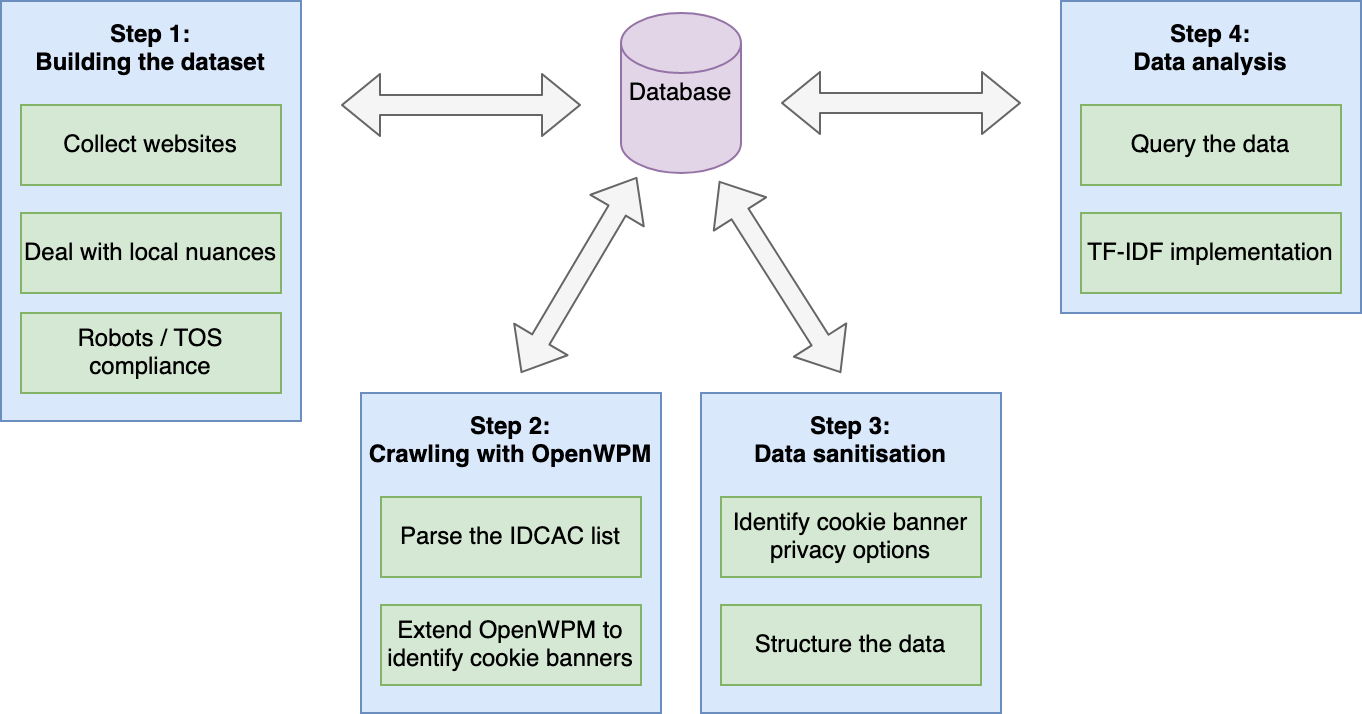
\includegraphics[width=\textwidth]{images/implementation/steps.png}
    \caption{The 4 implementation steps and their sub-tasks.}
    \label{fig:impl_steps}
\end{figure}

\end{document}